\documentclass[a4paper, 11pt, UTF8]{ctexart}
\usepackage{graphicx}
\usepackage{enumerate}
\usepackage{amssymb}
\usepackage{amsmath}
\usepackage{geometry}
\usepackage{caption}
\usepackage{subfigure}
\usepackage{float}
\usepackage{listings}
\usepackage{xcolor}
\usepackage{fontspec}
\usepackage{ulem}
\usepackage{hyperref}

\hypersetup{hidelinks}

\lstset{
    numbers=left,
    numberstyle= \tiny, 
    keywordstyle= \color{ blue!70},
    commentstyle= \color{red!50!green!50!blue!50}, 
    frame=shadowbox,
    rulesepcolor= \color{ red!20!green!20!blue!20} ,
    escapeinside=``,
    xleftmargin=2em, aboveskip=1em,
    framexleftmargin=2em,
    breaklines=true
}

\title{计算机程序设计基础大作业\\实验报告}

\author{机械108 \qquad 张益铭 \qquad 2021010552}

\date{2022年5月24日}

\geometry{left=3cm, right=3cm, top=4cm, bottom=4cm}

\begin{document}

\maketitle

\tableofcontents

\rightline{p.s. 点击目录进行跳转 :)}

\newpage

\section{实现功能及整体框架}

\subsection{实现功能}

本次大作业选题为大数计算器,实现了\textbf{基本功能}和\textbf{进阶功能},这两个功能在一个程序中实现。

其中,基本功能能够对用户输入的加、减、乘以及求余数($+, -, *, \% $)表达式进行计算,
数字的取值范围为int范围内的整形数字,最终结果需在long long范围内。

进阶功能是实现两个较大数字的乘法运算,对于较大的数字需要进行输入输出的重定向。

注:两种功能理论上能够计算任意长度的表达式,本程序中MAX\_SIZE取值为1000000,完全满足本次作业需求,
更改MAX\_SIZE的大小可以实现更大的计算。

\subsection{整体框架}

此次大作业代码模块化程度较高,主要分为输入处理部分、判断输入表达式合法性、基本功能的实现以及进阶功能的实现。
总共有一个*.h头文件和五个*.cpp源文件,总代码量为560行左右,使用GBK格式编码,注释、命名、分块较为合理。

\subsubsection{函数声明}

本次大作业使用的函数均在my\_function.h中进行声明,其中包含相关库的调用以及部分变量的声明,主要内容如下图所示。

\begin{figure}[H]
    \centering
    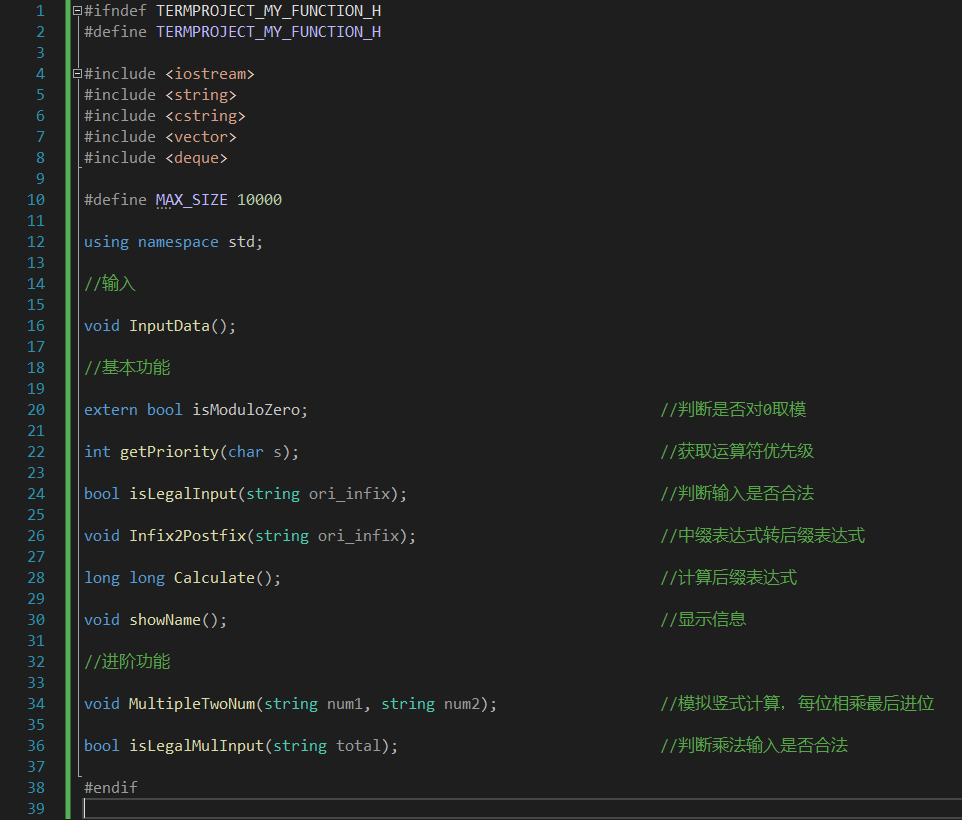
\includegraphics[width=0.7\textwidth]{my_function.png}
    \caption{my\_function.h}
\end{figure}

\subsubsection{主函数}

主函数main.cpp内容较简单,内含注释表明个人信息。main函数调用showName()和Input()函数,具体功能见后续介绍。

\begin{lstlisting}[language=C++, basicstyle=\ttfamily]
 //
 //Term Project of Programming Fundamentals.
 //Created by 张益铭 2021010552 on 4/13/2022.
 //Copyright (C) 张益铭 2022. All Rights Reserved.
 //Encoding with GBK.
 //

 #include "my_function.h"

 int main() {
    showName();
    
    Input();
    
    system("pause");
    return 0;
 }    
\end{lstlisting}

\subsubsection{输入处理}

输入处理工作主要由Input.cpp实现。

Input.cpp里的Input()函数(第3行)会对输入数据进行处理。用户需要先选择功能类型,1代表Basic Function(基本功能),2代表Advanced Function(进阶功能)。

随后程序会提示用户输入相应表达式,若表达式合法,就会调用相应的计算功能函数,否则会提示“Invalid function type!”。

\subsubsection{判断输入合法性}

判断输入合法性主要由Judgement.cpp实现。

Judgement.cpp中包含两个bool类型函数:isLegalInput()函数(第5行)和isLegalMulInput()函数(第91行),分别判断基本功能和进阶功能的表达式合法性。
若表达式合法,将会返回true并进行计算,否则会给出具体出错提示,并返回false。

\subsubsection{基本功能}

基本功能主要由BasicFunc.cpp实现。

包括getPriority()(第5行)、Infix2Postfix()(第22行)、Calculate()(第92行)、showName()(第145行)等函数,分别实现获取运算符优先级、
将输入的中缀表达式转化为后缀表达式、计算后缀表达式以及显示本人信息的功能。

\subsubsection{进阶功能}

进阶功能主要由AdvancedFunc.cpp实现。

包含Str2Int()(第3行)、MultipleTwoNum()(第59行)、getLen()(第131行)等函数,分别实现将字符串转化为分割后的数组,返回首位位置、计算两数相乘、
获取每组数字长度的功能。

\section{设计及实现思路}

\subsection{显示个人信息}

运行该程序后,先调用showName()函数,显示个人信息,该函数在BasicFunc.cpp中定义,较简单故不再赘述。

\begin{figure}[H]
    \centering
    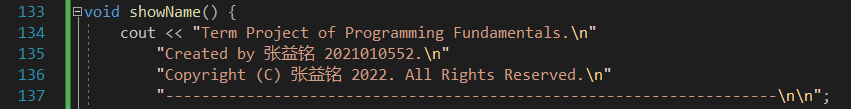
\includegraphics[width=\textwidth]{showname.png}
    \caption{showName()}
\end{figure}

其次调用Input(),处理输入。

\subsection{处理输入}

功能选择的合法的输入为1和2,对应基本和进阶功能。为区分不合法输入,本人使用string类变量whichFunc来记录用户选择,考虑到可能的错误如下:

\begin{enumerate}[a)]
    \item 输入字符串长度不为1
    \item 字符串长度为1,但不是1或2
\end{enumerate}

对于a,直接输出"Invalid function type!",程序结束;对于b,使用switch来扫描whichFunc[0],default项为输出"Invalid function type!"。

对于上述switch函数,case '1'为基本功能。
若表达式合法,即通过isLegalInput()的检验,再使用Infix2Postfix()将输入的中缀表达式转化为后缀表达式进行计算,
若运算中没有出现对0取余的情况,则输出结果res。

\begin{lstlisting}[language=C++, basicstyle=\ttfamily]
 case '1': {
    string ori_infix;

    cout << "Basic Func Mode.\n"
        "Please enter the expression:\n";
    getline(cin, ori_infix);

    if (isLegalInput(ori_infix)) {
        //表达式转换并计算
        long long res = Calculate(Infix2Postfix(ori_infix));
        if (!isModuloZero) {
            cout << "The result is:\n" << res << endl;
        }
    }
    break;
 }   
\end{lstlisting}

case '2'项对应进阶功能。
考虑到long long也装不下待计算数字,故定义string类变量num1和num2对应第一和第二个乘数。表达式通过isLegalMulInput()的检验后,会被分割为两个乘数。

由于输入后就删除了其中的空格,所以遇到*前使用.push\_back()存入第一个数,遇到*后开始存入第二个数。
关于是否到第二个数,我定义了bool类型变量isNum2来判断,部分代码如下。

\begin{lstlisting}[language=C++, basicstyle=\ttfamily]
 bool isNum2 = false;

 for (char i : total) {
    if (i == '*') {
        isNum2 = true;
    }
    if (!isNum2) {
        num1.push_back(i);
    }
    else if (i != '*') {
        num2.push_back(i);
    }
}
\end{lstlisting}

随后我申请了两块空间,用于存放分割后的数字,利用指针传递数组,最后进行计算。

\begin{lstlisting}[language=C++, basicstyle=\ttfamily]
 LongLongNum* num1_arr = new LongLongNum[MAX_SIZE];
 LongLongNum* num2_arr = new LongLongNum[MAX_SIZE];

 for (int i = 0; i < MAX_SIZE; ++i) {     //初始化
    num1_arr[i].s = 0;
    num2_arr[i].s = 0;
 }
 //获取倒序后最高位数字位置
 int num1_len = Str2Int(num1, num1_arr); 
 int num2_len = Str2Int(num2, num2_arr);

 MultipleTwoNum(num1_arr, num2_arr, num1_len, num2_len);

 delete[]num1_arr;
 delete[]num2_arr;
\end{lstlisting}

注:LongLongNum为my\_function.h中定义的结构体,用作存储long long类型的“数组”。

\begin{lstlisting}[language=C++, basicstyle=\ttfamily]
 struct LongLongNum { 
    long long s;
 };
\end{lstlisting}

\subsection{基本功能}

关于表达式合法性检测,我会在后文解释,现在我们假定输入均为合法输入。

考虑到中缀表达式并不利于计算机处理,并且受到PA08中3039后缀表达式作业的启发,我先将中缀表达式转化为后缀,再模仿栈的运行方式进行计算。

\subsubsection{获取运算符优先级}

由getPriority()完成。
由于遇到'('时入栈,直到遇到')'时将栈内运算符全部弹出,故定义'('优先级为1,'+'、'-'为2,'*'、'\%'为3,')'最高,为4,
并默认数字优先级为0。

\subsubsection{中缀转后缀}

由Infix2Postfix()完成。预处理:为了统一计算,我将正数改为0+本身,负数改为0-它的相反数,同时为了方便转化以及避免不必要的麻烦,
我在转化前遍历中缀表达式清除了其中的空格。

转化的主要思路是遍历中缀,遇到数字则存入后缀表达式,遇到运算符则存入vector容器op中,模拟栈的运行。

若遇到的运算符优先级小于上一个,则上一个运算符出栈,存入后缀,该运算符入栈,遍历完成后将栈内元素清空。
伪代码示意图如下:

\begin{figure}[H]
    \centering
    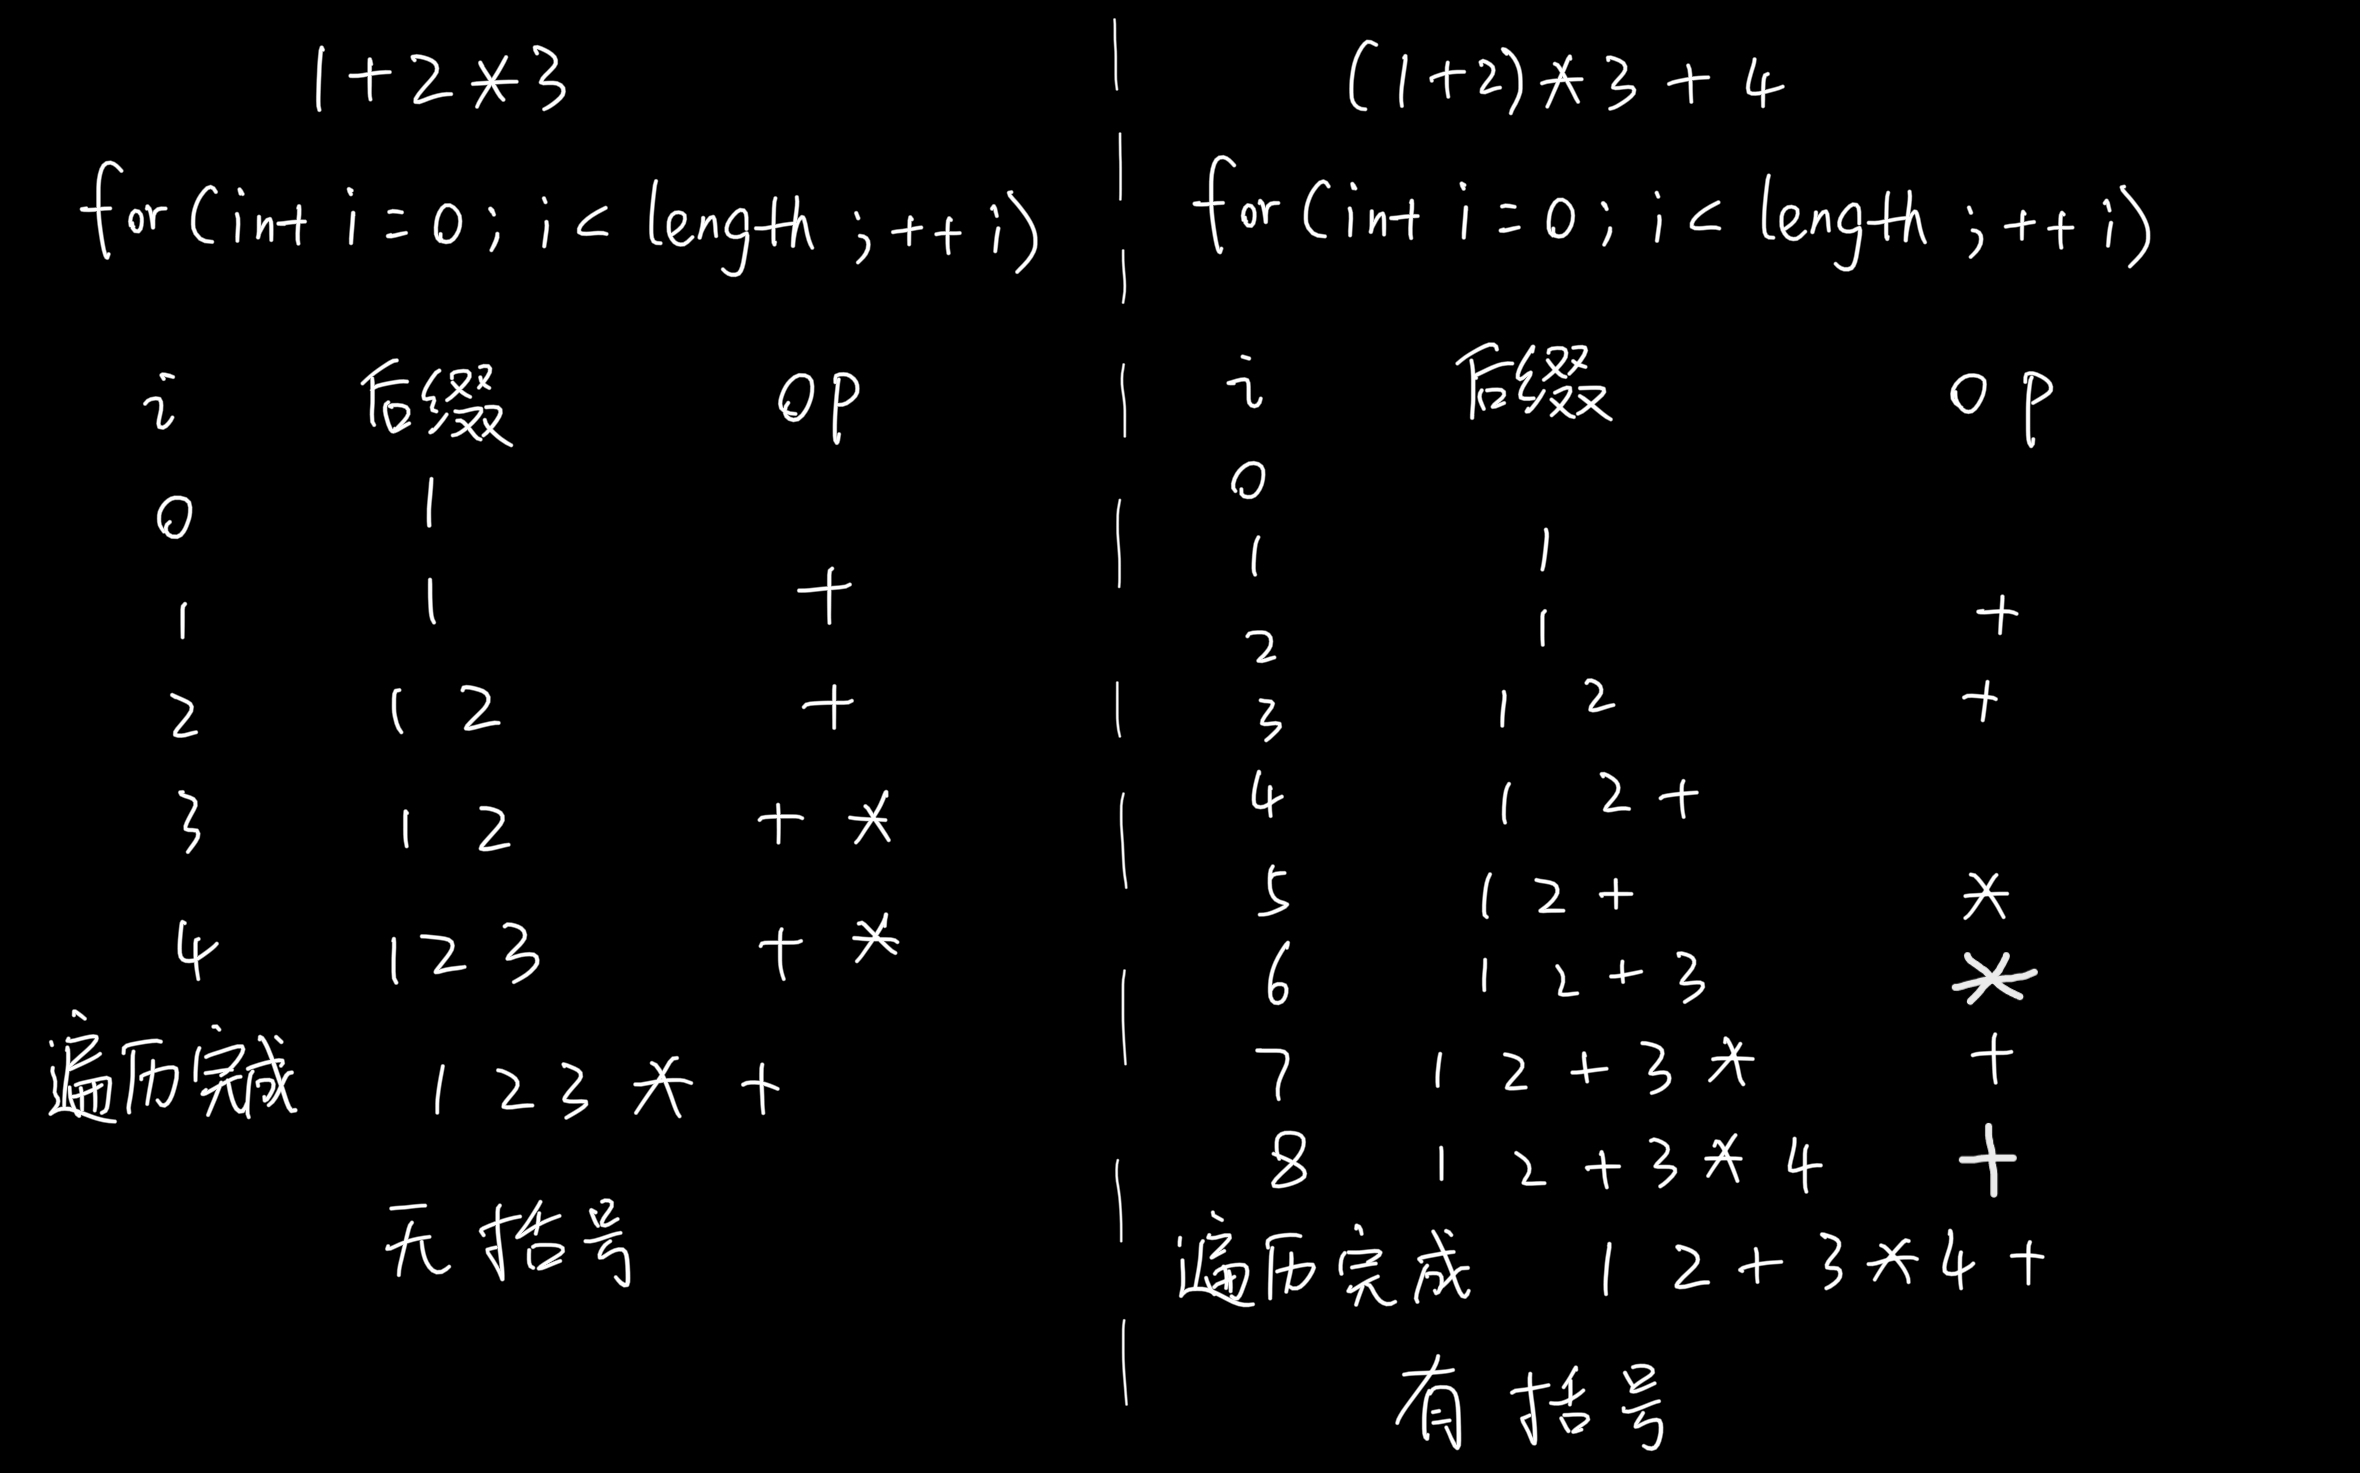
\includegraphics[width=0.8\textwidth]{infix2postfix.jpg}
    \caption{中缀转后缀示意图}
\end{figure}

\textit{*转化的后缀表达式存储在动态分配的数组postfix中。}

\verb|char* postfix = new char[MAX_SIZE];|

\subsubsection{计算后缀表达式}

由Calculate()完成。由于计算的结果在long long范围,int数组并不能满足,故我利用LongLongNum结构体存放stack变量:

\verb|LongLongNum* stack = new LongLongNum[MAX_SIZE];|。

思路是遇到数则压入栈中,遇到运算符则计算栈顶的前两个数字,栈顶元素出栈。
为防止对0取余,我定义了一个全局bool变量isModuloZero,检测到\%时判断栈顶元素是否为0,如果为0则将isModuloZero赋值为true,并输出“Modulo 0!”,
反之正常计算。

考虑到用户可能只输入一个数字,按照上述方法则不能输出该数字,所以在遍历完成时需检测num是否为0,若不是则将num作为结果输出。

\begin{lstlisting}[language=C++, basicstyle=\ttfamily]
 int j = 0;  //模拟控制入栈出栈
 for (int i = 0; i < strlen(postfix); ++i) {
    if (postfix[i] >= '0' && postfix[i] <= '9') {
        num = num * 10 + postfix[i] - '0';
    } else {
        if (num != 0 || (i >= 1 && postfix[i - 1] == '0')) {
            //防止负号前补充的0被忽略
            stack[j++].s = num;
            num = 0;
        }
        if (j >= 2) {
            ......  //进行运算
        }
    }
 }
 if (num != 0) {
    stack[j].s = num;
 }
\end{lstlisting}

\subsection{进阶功能}

进阶功能经历了两次大改,起初我模拟列竖式计算的过程,每次计算两个数位上的数字相乘,但这样计算复杂度太高,算到一万位乘一万位就已经超时了,具体如下:

\begin{lstlisting}[language=C++, basicstyle=\ttfamily]
 for (int i = 0; i < num1.length(); ++i) {
    for (int j = 0; j < num2.length(); ++j) {
        result[i + j] += (num1[i] - '0') * (num2[j] - '0');
    }
 }
\end{lstlisting}

后来我发现这种容器每个位置只存储了一位数字,利用率不高。由于long long类型范围为[-9223372036854775808,9223372036854775807],
能够\textbf{完整}表示18位数字,即两个九位数相乘的最大长度,因此我把待计算的数字每九位分为一个小节,一次相乘两个小节的数据,提高计算速度。

注:在本地测试中,更改算法后计算十万位乘十万位需要0.678000s,相比之前的22.375000s,极大地提升了运算速度(不同电脑测试时间略有差异)。

\subsubsection{数据分割}

为了防止相乘后数字进位导致头部溢出,我将数字倒序分割,最后九位放在arr[0],头部放在arr结尾,以此类推。例如12123456789987654321就被分割为了
\begin{table}[H]
    \centering
    \begin{tabular}{ccc}
        \hline
        \multicolumn{1}{|c|}{987654321} & \multicolumn{1}{c|}{123456789} & \multicolumn{1}{c|}{12} \\ \hline
        arr{[}0{]}                      & arr{[}1{]}                     & arr{[}2{]}
    \end{tabular}
\end{table}

主要思路为对于能被分割的部分,相应数位乘十亿、一亿、一千万等组合成一个数字,然后将结果放入数组中,对于不够九位的部分再具体分析。

最后,还要注意头部可能存在0,譬如输入00000123456789,就需要去除首位的0,返回正确的首位位置。

\subsubsection{计算两数相乘}

首先我申请了一块空间用于存储结果

\verb|LongLongNum* res = new LongLongNum[MAX_SIZE];|

主要计算思路依然类似于竖式乘法,只不过竖式乘法每次乘两位数字,这里每次乘两个小节的数字。
具体实现依旧是各个数位交叉相乘,乘完一组后直接向上进位,核心代码如下:

\begin{lstlisting}[language=C++, basicstyle=\ttfamily]
 for (int i = 0; i < num1_len; ++i) {
    carry = i;
    for (int j = 0; j < num2_len; ++j) {
        res[carry].s += num1[i].s * num2[j].s;  //交叉相乘
        if (res[carry].s >= 1000000000) {
            res[carry + 1].s += res[carry].s / 1000000000;
            res[carry].s %= 1000000000;         //进位
        }
        ++carry;
    }
}
\end{lstlisting}

还需注意的是每组数据是用long long而不是string保存的,因此如果中间数位不足9位,则需要补0,否则会出现缺0的情况。
所以我写了一个简单的函数getLen()来获取每小节数字长度,该函数如下:

\begin{lstlisting}[language=C++, basicstyle=\ttfamily]
 int getLen(long long num) {
    int len = 0;
    while (num > 0) {
        num /= 10;
        ++len;
    }
    return len;
 }
\end{lstlisting}

除去首位后(首位无需补0),如果res[i]的长度小于9,则需要先输出对应多个0,然后再输出res[i],保证结果准确性。

\subsection{程序鲁棒性}

\sout{众所周知,写代码5分钟,debug两小时},为了避免各种可能的异常输入导致程序崩溃,我想到了如下了可能出现的异常。

\begin{table}[H]
    \centering
    \begin{tabular}{|ccc|}
        \hline
        \multicolumn{3}{|c|}{\textbf{可能的输入异常}}                                           \\ \hline
        \multicolumn{1}{|c|}{}  & \multicolumn{1}{c|}{\textbf{基本功能}}    & \textbf{进阶功能} \\ \hline
        \multicolumn{1}{|c|}{1} & \multicolumn{1}{c|}{是否输入}             & 是否输入          \\ \hline
        \multicolumn{1}{|c|}{2} & \multicolumn{1}{c|}{第一位不是数字}       & 乘数个数          \\ \hline
        \multicolumn{1}{|c|}{3} & \multicolumn{1}{c|}{英文/中文符号}        & 乘号个数          \\ \hline
        \multicolumn{1}{|c|}{4} & \multicolumn{1}{c|}{输入不是数字}         & 是否是乘号        \\ \hline
        \multicolumn{1}{|c|}{5} & \multicolumn{1}{c|}{缺少/多余/错误运算符} & \textbackslash{}  \\ \hline
        \multicolumn{1}{|c|}{6} & \multicolumn{1}{c|}{多/少括号}            & \textbackslash{}  \\ \hline
        \multicolumn{1}{|c|}{7} & \multicolumn{1}{c|}{对0取余}              & \textbackslash{}  \\ \hline
    \end{tabular}
\end{table}

注:为了避免不必要的麻烦,两种功能都会删除表达式中的空格。遇到任何一种错误都会给出提示并返回false,
只有通过全部检验才回返回true,进行后续计算。

\subsubsection{基本功能输入异常}

基本功能需考虑的异常相对较多,我将按照上表依次介绍相关处理思路。

\begin{enumerate}
    \item 对于是否输入,只需检测长度是否为0,若为0,立即显示“Please enter the expression!”,程序结束。
    \item 一般情况下,表达式中第一位都是数字或者括号,因此若第一位是“*,\%”中的任一种,
          都会提示“Operator missing operand!”。但是只输入一个符号也是不行的,因此如果表达式长度为1并且第一位是符号也会报错。
    \item 由于计算表达式中含有括号,部分用户可能输入中文输入法下的括号,造成输入异常。经测试知,‘(’和‘(’对应的ASCII码并不相同,
          中文每个汉字由两个及以上字节组成,具体表现为其ASCII码小于0,因此在遍历过程中遇到某位的ASCII码小于0
          就会提示“Please enter expressions in English!”
    \item 当输入不是数字时,则必须是合法运算符中的一种,所以在遍历中使用了switch函数判断输入不是数字的情况。
          \begin{lstlisting}[language=C++, basicstyle=\ttfamily]
if (ori_infix[i] < '0' || ori_infix[i] > '9') {
    switch (ori_infix[i]) {
        case '(':
        case ')':
        case '+':
        case '-':
        case '*':
        case '%':
            break;
        default:
            cout << "Invalid operator!\n";
            return false;
    }
}
          \end{lstlisting}
    \item 对于输入运算符错误,可能的情况有:连续多个加减乘取余符号、除了正负号之外的左括号连接运算符(不包括连续多个左括号)、
          运算符连接右括号(不包括连续多个右括号)等问题,发现任意一种都会输出“Operator missing operand!”
    \item 多/少括号的判断则比较简单,只需统计左右两种括号的个数,二者不相等就会输出“Parenthesis DO NOT match!”
    \item 关于判断是否对0取余,已经在Calculate()中进行了介绍,不再赘述。
\end{enumerate}

\subsubsection{进阶功能输入异常}

进阶功能输入异常相对较少,主要如下。

\begin{enumerate}
    \item 对于是否是输入,处理方法同基本功能。
    \item 若第一位是'*',说明未输入第一个乘数,会提示“Please enter the first multiplier!”,如果表达式最后一位是'*',
          说明未输入第二个乘数,提示“Please enter the second multiplier!”
    \item 统计乘号个数,如果不是1则提示“You can ONLY multiply two numbers!”
    \item 由于进阶功能的输入只有数字和乘号,所以对于数字之外的输入,如果是乘号,则乘号个数+1,
          否则输出“Invalid signs!”
\end{enumerate}

\section{使用说明及实现效果}

注:相关输入要求见readme.txt

\subsection{开始}

首先,程序会提示用户选择功能类型(1代表Basic Function,2代表Advanced Function).

\begin{figure}[H]
    \centering
    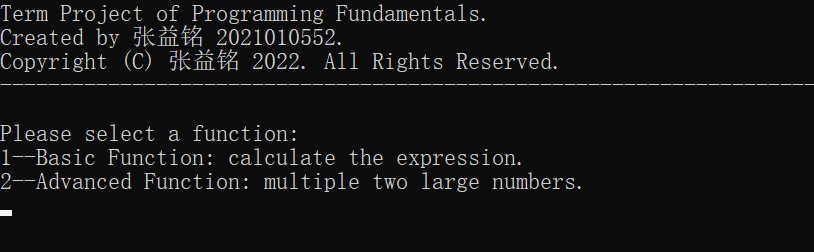
\includegraphics[width=0.96\textwidth]{begin.png}
    \caption{选择功能}
\end{figure}

选择完毕后程序会显示当前的功能,并提示输入表达式。

\begin{figure}[H]
    \centering
    \begin{minipage}[t]{0.48\textwidth}
        \centering
        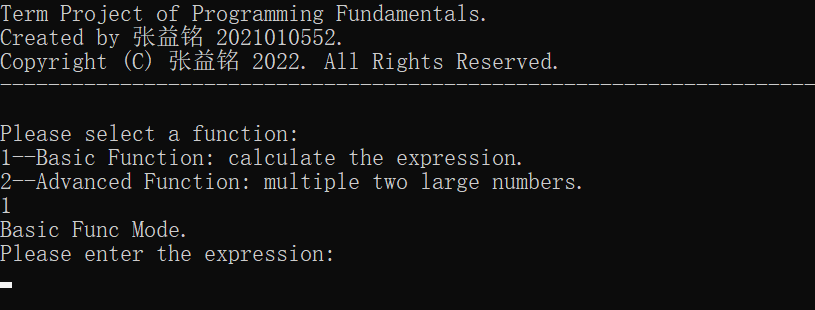
\includegraphics[width=7cm]{func1.png}
    \end{minipage}
    \begin{minipage}[t]{0.48\textwidth}
        \centering
        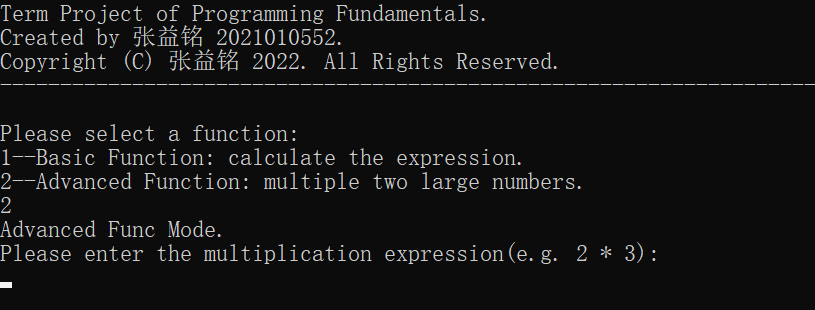
\includegraphics[width=7cm]{func2.png}
    \end{minipage}
    \caption{两种功能页面}
\end{figure}

\subsection{功能1:基本功能}

用户在基本功能里可以输入加、减、乘、取余表达式,能够进行括号运算,数字内部不可以有空格,两个数之间可以有任意数量的空格,
输入完成按下enter后,会显示“The result is:”并输出结果,部分输入结果如图。

\begin{figure}[H]
    \centering
    \subfigure{
        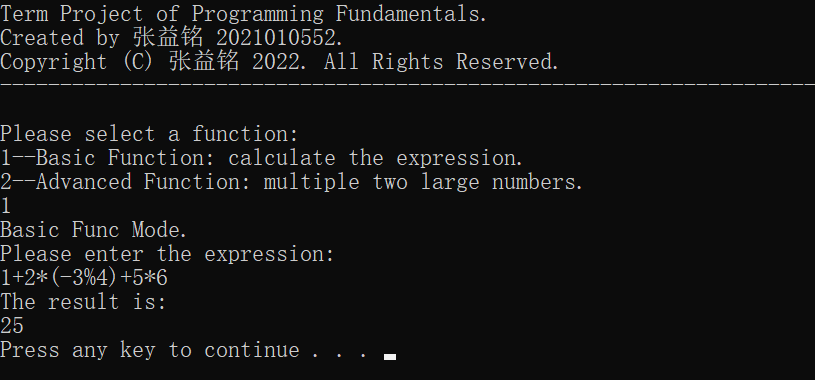
\includegraphics[width=0.65\textwidth]{res11.png}
    }
    \quad
    \subfigure{
        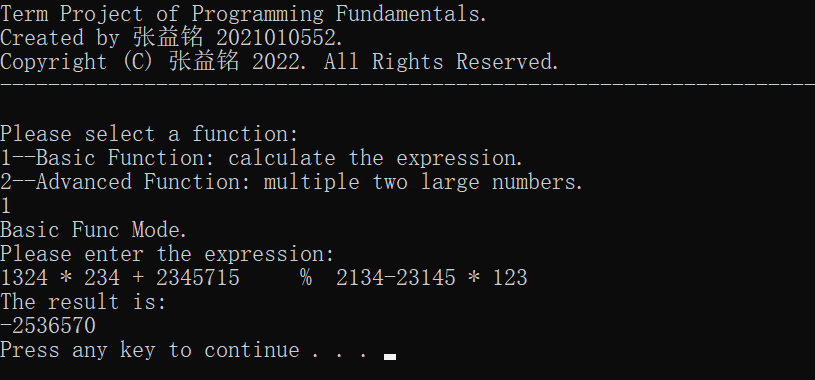
\includegraphics[width=0.65\textwidth]{res12.png}
    }
    \quad
    \subfigure{
        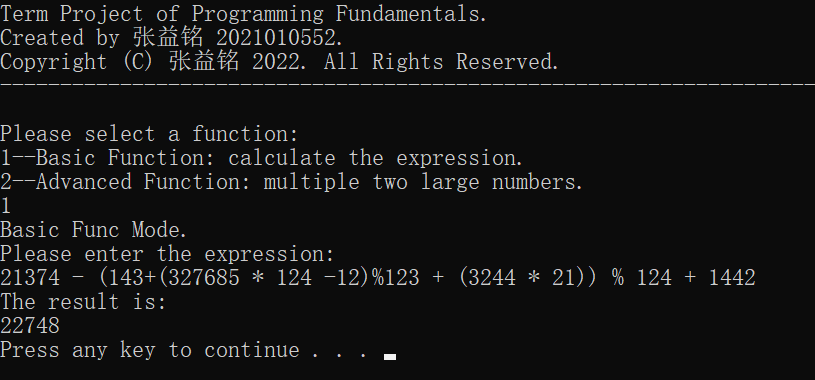
\includegraphics[width=0.65\textwidth]{res13.png}
    }
    \quad
    \subfigure{
        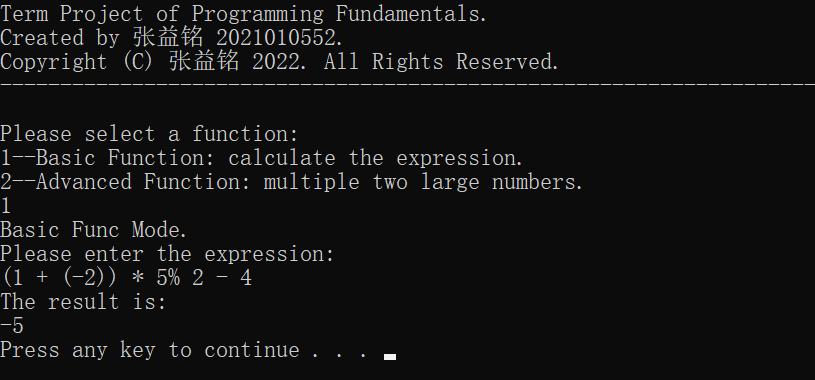
\includegraphics[width=0.65\textwidth]{res14.png}
    }
    \caption{部分输入案例}
\end{figure}

\subsection{功能2:进阶功能}

进阶功能用户可计算两个大数的乘法,其中数字的位数应该在int范围内(远远满足作业100000位的要求),且两个数应均为非负数,
输入完成按下enter后,会显示“The result is:”并输出结果,部分输入结果如图。

\begin{figure}[H]
    \centering
    \subfigure{
        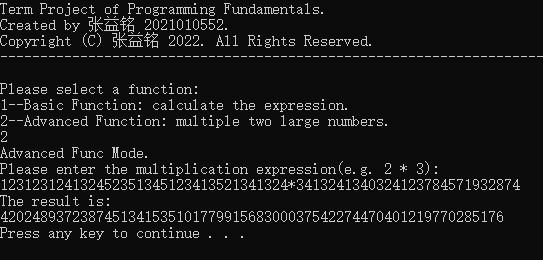
\includegraphics[width=0.7\textwidth]{res21.png}
    }
    \quad
    \subfigure{
        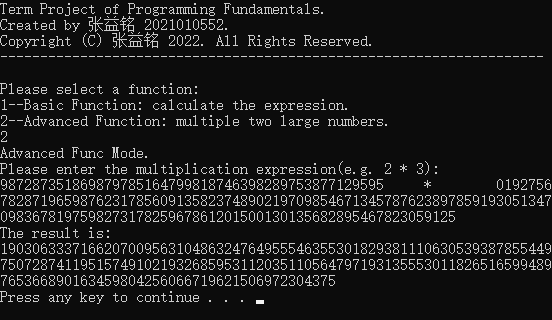
\includegraphics[width=0.7\textwidth]{res22.png}
    }
    \quad
    \subfigure{
        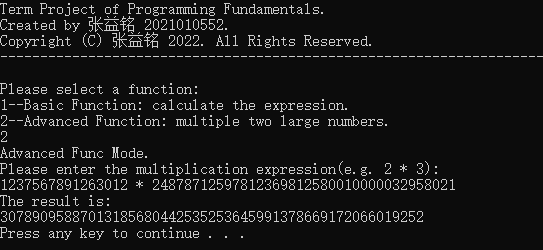
\includegraphics[width=0.7\textwidth]{res23.png}
    }
    \caption{部分输入案例}
\end{figure}

\end{document}
